\section{Further reviewer revisions: scale and causal controls}
We retain the original correctness intervention, collision construction, complete-logit invariant swaps, and orbit exclusion. A post-confirmation census evaluates every unexposed orientation in each source's remaining 511--530 orbits, totaling 3,066--3,180 inputs per source. Independently paired collision inputs agree on all three visible gold answers and disagree on the compound answer. Each input is used once; complete orbits can recur across pairs. These are larger tests of old models, not new source/world replications.

\begin{table}[ht]\centering\small
\begin{tabular}{lrr}\toprule Condition & Accuracy (\%) & Both (\%)\\\midrule
nonlinear correct & 17.94 & 3.24 \\
nonlinear wrong & 7.46 & 0.48 \\
linear correct & 8.53 & 0.73 \\
linear wrong & 8.03 & 0.40 \\
affine correct ols initialization & 17.86 & 2.95 \\
affine wrong ols initialization & 7.44 & 0.53 \\
validation selected ridge correct & 11.19 & 1.19 \\
validation selected ridge wrong & 7.75 & 0.38 \\
\bottomrule\end{tabular}
\caption{Expanded gold-matched collision subset, averaged over the five old sources. Orbit dependencies remain.}
\end{table}

\paragraph{Equivalence remains secondary.}
On the complete orbit census the unregularized affine--GELU difference is 0.237pp; the descriptive 90\% source interval is $[-1.000,1.475]$pp. A posthoc paired TOST rejects non-equivalence for $\pm3$pp, whereas the original smaller test did not. This does not establish prospective equivalence on new data worlds. Normal-model planning with the old SD of 5.35pp requires 29 independent units for $\pm3$pp and 12 for $\pm5$pp at 80\% power if the true mean is zero; a 1pp true mean raises these to 46 and 14. The old variance is not a variance estimate for the new world. All equivalence analyses are secondary to the functionality question.

\paragraph{Ridge sensitivity weakens a broad optimization conclusion.}
We penalize standardized affine input coefficients, leaving the intercept unpenalized, and fit the same teacher-KD plus normalized-state objective with this added term. The ridge path is fixed before new predictions and selected only on known validation states/logits. Functional accuracy falls as small directions are suppressed; validation-selected fits perform poorly. Thus recovery by the unregularized solution is not robustly demonstrated under ordinary validation-selected regularization. This changes the empirical objective and cannot invalidate the original unregularized optimum certificate. The source of useful small directions remains unresolved.

\paragraph{Natural-state interchange is informative but not an ideal control.}
Balanced donor permutations preserve gold first answers and marginal donor frequency. With a distinct second answer, the natural donor is followed in 56.89\% of cases. With the same second answer, only 82.13\% remain correct and 18.25\% change predictions. All tested first-step logits remain invariant. The substantial same-answer disturbance fails the proposed near-invariant control, and natural components do not guarantee natural hybrids. The evidence supports downstream answer-information transport under the specified intervention, rather than natural mathematics-specific causal encoding. Geiger et al.'s interchange framework motivates the stronger prospective control \cite{geiger2021causal}.

\paragraph{A new-world confirmation is kept separate.}
The following section reports the completed frozen $\F_{17}$ experiment. Those independent dataset/source units are distinguished from the posthoc old-world census above. The interface-only parameter-count amendment was made before first-operator fitting or new composite evaluation, with both protocol versions retained. Failed performance and interchange gates are reported rather than used to replace units.

\begin{figure}[ht]\centering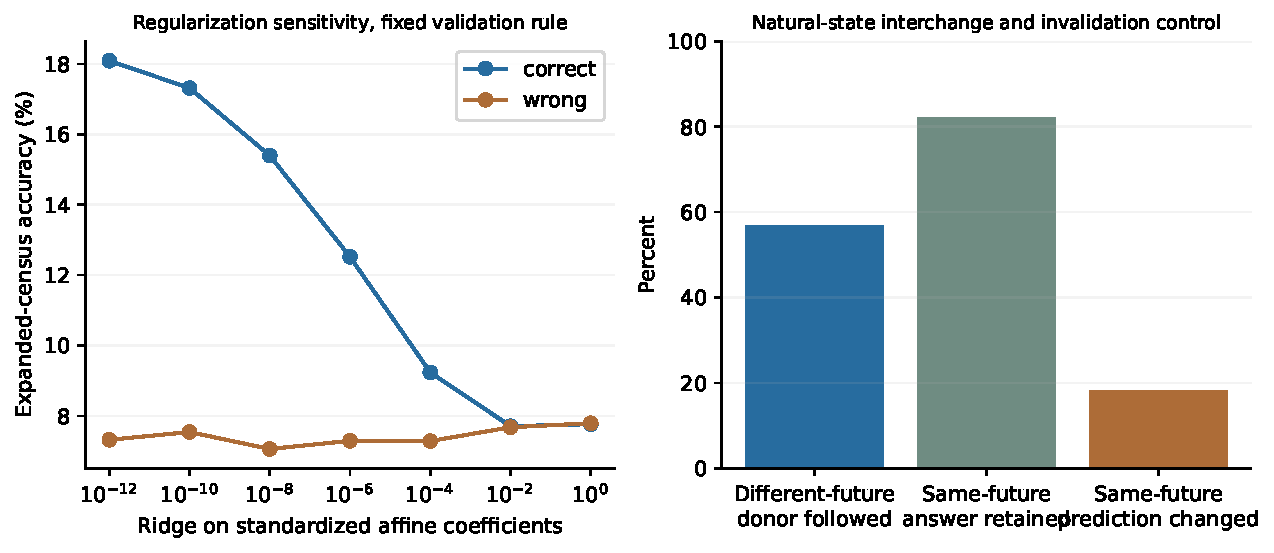
\includegraphics[width=\linewidth]{figures/reviewer_revision.pdf}
\caption{Complete-census regularization sensitivity and natural-state interchange. The same-answer disturbance prevents an unqualified causal-mechanism claim.}
\end{figure}
